%%%%%%%%%%%%%%%%%%%%%%%%%%%%%%%%%%%%%%%%%%%%%%%%%%%%%%%%%%%%%%%%%%%%%%%%%%%%%%%%
%2345678901234567890123456789012345678901234567890123456789012345678901234567890
%        1         2         3         4         5         6         7         8

\documentclass[letterpaper, 10 pt, conference]{ieeeconf}  % Comment this line out if you need a4paper

%\documentclass[a4paper, 10pt, conference]{ieeeconf}      % Use this line for a4 paper

\IEEEoverridecommandlockouts                              % This command is only needed if
                                                          % you want to use the \thanks command

\overrideIEEEmargins                                      % Needed to meet printer requirements.

% natbib hack
% http://newsgroups.derkeiler.com/Archive/Comp/comp.text.tex/2006-02/msg00834.html
\makeatletter
\let\NAT@parse\undefined
\makeatother
\usepackage[numbers]{natbib}

% The following packages can be found on http:\\www.ctan.org
\usepackage[pdftex]{graphicx}
\usepackage{amsmath} % assumes amsmath package installed
\usepackage{amssymb}  % assumes amsmath package installed
\usepackage{subfigure}
\usepackage{multirow}
\usepackage{array,booktabs}
\usepackage{diagbox}
\usepackage{balance}
\usepackage{amsmath}
\usepackage[ruled,vlined]{algorithm2e}
\usepackage{algpseudocode}
\usepackage[export]{adjustbox}
\usepackage{caption}
\usepackage{hyperref}
\usepackage{textcomp}
\usepackage{ctable}

\usepackage{irap_SIunits}
\usepackage{irap_acronyms}
\usepackage{irap_math}
\usepackage{irap_misc}

% for comments
\usepackage{soul,color}

% To highlight the revised MS
\usepackage{xcolor}
\newcommand{\bl}[1]{{\textcolor{blue}{#1}}}
\newcommand{\gr}[1]{{\textcolor{green}{#1}}}
\newcommand{\fl}[1]{{\textcolor{red}{#1}}}
\newtheorem{theorem}{Theorem}

\DeclareMathOperator*{\argmin}{arg\,min}
\DeclareMathOperator{\Tr}{Tr}

\begin{document}
\title{\LARGE \bf
	Continuous Trajectory Estimation from Depth Augmented Events
}

\author{Alex Junho Lee$^{1}$, Jinyong Jeong$^{1}$, Younggun Cho$^{1}$, Sungho Yoon$^{2}$, Young-Sik Shin$^{3}$, and Ayoung Kim${}^{1,2*}$
	%\thanks{*\hl{Need ack.}}% <-this % stops a space
	\thanks{$^{1}$Department of Civil and Environmental Engineering,
		\acs{KAIST}, 291 Daehak-ro, Yuseong-gu, Daejeon 34141, Republic of Korea
		{\tt\small [alex\_jhlee,jjy0923,yg.cho,ayoungk]@kaist.ac.kr}}%
	\thanks{$^{2}$Robotics Program,
		\acs{KAIST}, 291 Daehak-ro, Yuseong-gu, Daejeon 34141, Republic of Korea
		{\tt\small sungho.yoon@kaist.ac.kr}}%
	\thanks{$^{3}$ Korea Institute of Machinery and Materials
		Daejeon 34141, Republic of Korea
		{\tt\small yshin86@kimm.re.kr}}%
}


\maketitle

\thispagestyle{empty}
\pagestyle{empty}


\begin{abstract}

Event cameras have arisen as an alternative solution to trajectory estimation problem
on real-world applications, by its consistent sensor measurement upon environmental variance.
In this paper, we present a method of estimating a continuous trajectory from event measurements
combined with a depth sensor. We combine sequential depth information with continuous
event stream to estimate a 6 DOF trajectory. From accurate depth measurements from the
infrared depth sensors or solid-state LiDARs, edge structures are extracted and fitted
into the events to estimate a polynomial spline trajectory. We show that to fully utilize
the benefits from continuous-time representation of events, camera localization should
be solved as a continuous trajectory estimation problem. We also release a public dataset
including dynamic lighting conditions and various motion
in indoor and outdoor, with ground-truth provided. The dataset can be downloaded from : 
\url{https://sites.google.com/view/vivid-kaist}
\end{abstract}

\section{Introduction}
\label{sec:Event}

Neuromorphic vision sensors, also known as \ac{DVS} \cite{lichtsteiner2008128x128} has been proposed as an effective alternative of vision sensor from its several advantages over regular cameras. Frame-based imaging sensors produce an image, which is time-synchronized scene data during exposure time. The sequential output known as image data is intuitive and effective for \ac{VO} \cite{forster2014svo} and \ac{SLAM} \cite{mur2017orb} even with a single camera. And the sensor measurement is produced by integrating a number of photons arrived during the exposure time, requiring specific duration for every measurement. Therefore, image data has limits of the trade-off between frame-rate and dynamic range and is not able to sense changes occurred in exposure time. However, event cameras are free from the problems of classic ones. Neuromorphic vision is not based on the number of photons integrated for a duration but measures the rate of a photon entering each pixel. Therefore, event cameras avoid temporal integration and retain asynchronicity with high dynamic range (up to $130dB$, which is significantly higher than the $60dB$ of conventional cameras).

Since the event camera possesses an asynchronous \ac{AER} representation of illumination change, data acquired from event cameras are not demonstrated with discrete timings. To fully utilize the unique \ac{AER} of event camera, any information obtained from the event camera should be dealt with as a continuous-time problem. However the number of events may sum up to millions per second, raising temporal sampling resolution does not solve the problem, yielding heavy computation load. Therefore event requires a total new way of data processing.

\begin{figure}%
	\centering%
	\includegraphics[width = \columnwidth]{figures/figure1small}%
	\captionsetup{justification=centering}
	\caption{Estimated trajectory and reconstruction from events \protect\linebreak with depth (left), Iterative
		Closest Points (ICP) on depth pointclouds (right). Trajectory estimation using only depth fails on extreme motion, as demonstrated in white circle.}%
	\label{F:main}%
	\vspace{-5mm}
\end{figure}

Thus event cameras related researches have focused on finding a way on processing temporal information while less degenerating data. Since pose representation enables global optimization techniques like bundle adjustment or pose-graph, majority of research in event-based \ac{VO} has been examined on transforming continuous signal into subsequent pose form \cite{lagorce2015asynchronous}, \cite{clady2015asynchronous}, \cite{weikersdorfer2012event}, \cite{kim2016real}. However, sequential procedures of classical image processing such as feature extraction, descriptor matching with calculating re-projection error were not necessary for event-based algorithms if the pose is not in a discrete representation \cite{rebecq2017evo} \cite{vidal2018ultimate}. Despite the idea of directly fitting motion from event measurements were in a proper way of utilizing the benefits of event cameras, its relatively lower spatial resolution and noise made it difficult to use events as a single origin pose estimator. To deal with this problem, we suggest combining sparse sensor measurements with events, while maintaining continuous pose representation as a trajectory.

In this paper, we aim to solve the motion estimation problem with the benefits of event sensors by:
%

\begin{itemize}
	\item Solving motion estimation problem by estimating polynomial spline trajectory from finding correspondence of continuous events between depth measurements

	\item Defining correspondence between events and disjointly updated depth, by associating depth discontinuity into event generating edges in the image domain.
	
	\item Releasing a first public dataset to cover illumination and motion variances by multi-modal sensor
	measurements consisted with event, depth, and thermal camera.

\end{itemize}

%---------------------------------------------------------------------------%
\section{Related Works}
\label{sec:related}

\subsection{Event-based Visual Odometry}

The unique advantages of \ac{AER} and event cameras have encouraged researchers to solve motion estimation aided by event measurements. Since event cameras have both advantages and challenges as described in the previous section, researchers have developed several ways of defining relationship between events, that are continuously measured but asynchronous to typical discrete pose representations.

In the early stages, researchers established probabilistic approaches on event-based \ac{VO}. A method that first succeeded involves calculating posterior probability with a temporal threshold. \citeauthor{kim2008simultaneous}~\cite{kim2008simultaneous} has introduced to use \ac{EM} schema on fitting events for upon rotational motion. This study was expanded to the optimization of 6-\ac{DOF} trajectory with 3D reconstruction \cite{kim2016real}. Their approach has revealed the way of directly optimizing the trajectory from events, yet was filter-based and had less robust due to numbers of assumptions. In \cite{weikersdorfer2012event}, authors implemented a particle filter to minimize ray distance through all features in 2D. This study was broadened to include 3D \ac{SLAM} in \cite{weikersdorfer2013simultaneous}, but was only effective in planar scenes.

On the other hand, there was another approach reminding of \ac{SAE} introduced in \cite{adelson1985spatiotemporal}. \cite{mueggler2015lifetime} fitted a surface in an $\mathcal{XYT}$ space with \ac{SAE} to estimate the effective temporal length for each event. These studies suggested finding the effective size of the temporal window and to only filter relevant events with adaptive temporal window size. The proposed algorithm provides a hint for utilizing the high temporal resolution characteristics of events by processing with individual timings.

In \cite{ieng2018neuromorphic}, a modified version of \ac{SAE} with exponentially decaying kernels was introduced for \ac{VO}. In this study, events are accumulated in exponential time-surface and calculated for an optimal camera pose by optimizing re-projection error with other measurement models in stereo-vision. The study focused on directly estimating the camera pose with exponentially decaying kernels, which provided a smoothed representation of \ac{SAE}. The authors introduced a robust descriptor of \ac{SAE} in addition to filtering with tree assignment. As a result, the author was able to enhance the mean tracking frequency on the scale. Although their work is based on the complex model and the user-defined descriptor, it has shown that calculating from each event's timestamp could arrange to a convergence.

The next was generating motion-related frame images by temporal thresholding. Numbers of researches had set effective events within a fixed time interval and tried to build event images for discrete trajectory estimation. However, this procedure integrates the asynchronous event signals into synchronous sequences with a fixed temporal window, resulting in the loss of piecewise timing information on each event. Therefore in order to achieve higher levels of accuracy and fully utilize the temporal resolution of event cameras, another solution were required than simple thresholding.

Several studies attempted to utilize the high temporal resolution of event cameras by assigning proper weights to each event. \citeauthor{gallego2017accurate}~\cite{gallego2017accurate} introduced a direct method of accurately estimating angular velocity by compensating events for rotational motion. This approach was the first attempt to build a motion-compensated event frame, that could both conserve asynchronicity and frame-based odometry estimation. In combination with nonlinear optimization, \cite{rebecq2017real} succeeded in integrating \ac{IMU} for 6 \ac{DOF} event \ac{VO}. This study demonstrated a standard pipeline for event-based \ac{VINS}. Although this approach became robust and effective by enabling classical feature-based methods on an event stream, the requirement of generation procedure on the motion-compensated event image for every pose and extracting features demands proper initialization.

\citeauthor{mueggler2018continuous}~\cite{mueggler2018continuous} proposed a method of optimizing the trajectory with events and \ac{IMU} by introducing cubic spline interpolation into \cite{rebecq2017evo}. Ultimate SLAM \cite{vidal2018ultimate} was nonetheless the state-of-the-art method for integrating sensor measurements with motion-compensated event frames. However, the proposed algorithm required updating the spline parameter upon receiving each event, which was quite heavy in computation.

In this research, we introduce a method to estimate polynomial continuous trajectory in 3D,
by directly optimizing spline parameters efficiently with continuous event measurements and
sparsely obtained depth measurements.

\subsection{Datasets for Environmental Variance}

Numbers of datasets for benchmarking \ac{SLAM} has been introduced
\cite{Cordts2016Cityscapes}, \cite{jjeong-2019-ijrr} with
clear sight and high visibility. Meanwhile, in the real world, lighting
conditions are often uncooperative, making computer vision algorithms fail.
Moreover, there are few of datasets made to test experimental
environments with environmental variations.

NCLT \cite{ncarlevaris-2015a} and TUM MonoVO \cite{engel2016photometrically}
introduced large scale data with huge variance in environments for long-term visual
\ac{SLAM}. These datasets cover challenging indoor and outdoor sequences including
natural light and weather changes. However, obtaining the limited information from the
classical camera restricts the bandwidth of data from the environment, skipping
potentially important information.

By using other types of visual sensors, Choi et al. \cite{8293689} presented
a multi-spectral day/night dataset with the sensor set of stereo RGB, LiDAR and
a thermal camera. Their data contains variance along the whole day. Furthermore,
numbers of labeled data are provided for autonomous navigation.
However, camera movements in the dataset are limited to planar motion because the
system is mounted on a car.

In \cite{zhu2018multivehicle}, the authors have presented a dataset measuring
various lighting and motion sequences with two event cameras aligned with
inertial sensors and an \ac{IMU}. The dataset contains a large variety of
condition changes, suggesting utilizing the event camera for low latency and high
dynamic range characteristics.

Although several datasets have contained environmental variations
including movement or lighting variances, unspecified natural environment often
possess both of them. In this paper, we release a dataset to record both thermal
and events with depth in order to deal with two significant disturbances:
luminance conditions and motion. Along the dataset, we also suggest the method to
estimate polynomial continuous trajectory in 3D, thereby directly optimizing spline\
parameters efficiently with given depth measurements.

\section{Method}
\label{sec:method}

%ALGO
\begin{algorithm}[!b]
\SetAlgoLined
	\KwData{Single depth image, event stream}
	\KwResult{6 dof continuous trajectory}
	$\ $\\
	$X_{depth}$ = Extracted edge cloud from depth image\;
	$T_e$ = Tree structure built from events\;
	$\ $\\
	\Repeat{Converge}{
		build polynomial spline trajectory $P(v)$\\
		\For{number of intervals}{
			$X'_{depth}$ = transformed $X_{depth}$ with $P(v)$\\
			$I$ = projected points of $X'_{depth}$ on event frame\\
			search nearest neighbour of $I$ from $T_e$\\
			update loss \eqref{eq:loss}
		}
		update spline parameters $v$\\
	}
	\caption{Continuous polynomial spline trajectory estimation with
		depth image and events}
\end{algorithm}
%ALGO

In our method, we start from depth measurement and preprocess the depth image with
an edge detector to extract structural edges. As events are only generated upon
changes in luminance, measurements occurred from event camera are all from photometric
and geometric edges. Thus assuming enough structural than color difference, projected
depth edges could be matched to event measurements.

Depth cameras, such as Kinect or Xtion, provide accurate depth information with
resolution of millimeters in indoor environments. However it may fail to match between
measurements with large baseline, since the sensor rate usually is around tens of hertz.
Robotic systems like drones could generate aggressive motion in real world, thus relying
on single frame-based sensor may be vulnerable. To overcome this problem, we suggest to
find relative motion from another sensor with higher frame, which is event camera.
Our algorithm is to utilize the continuous measurement characteristics of event camera,
to estimate the motion occurred between frames of the depth sensor.

From measurement obtained with depth camera, we may transform the pointcloud into
event camera's frame, and project them into image plane. Then the depth image from
event frame is obtained, we use using edge detectors for detecting geometrical
discontinuities in the image. Although sensors are placed closely, there are
occlusions and discontinuities due to occluded area should be ignored. For
transforming depth measurements into event camera frame, we used extrinsic
calibration provided from the dataset released.

After extracting geometric discontinuities from event frame with depth camera,
we define a polynomial spline and recursively update basis parameters to minimize
the loss. We defined loss as weighted sum of three losses : distance between
geometric edge and incoming events, error of reprojected depth measurements and
parameter regularization term.
\begin{eqnarray}
\label{eq:loss}
L &=& L_{struct} + L_{endpose} + L_{param}\\
L_{struct} &:& \text{Structure matching loss}\nonumber\\
L_{endpose} &:& \text{End pose loss}\nonumber\\
L_{param} &:& \text{Regularization loss}\nonumber
\end{eqnarray}
Given spline parameter $v$ with n variables, we construct polynomial trajectory
with nth order basis function $P_n(t,v)$, where $v$ is polynomial spline parameter, as
\begin{equation}
P_n(t,v) = \sum_{i=1}^{n} v_i t_i \nonumber
\end{equation}
where t is time between two depth poses. Note that there's no zeroth order term
from we're solving relative pose problem, so $P(0,v)=0$. Then with this 6dof
polynomial curve, we may transform the geometrical edge point $X_{depth}$ and find nearest
neighbour from built tree structure of events $T_e$.
\begin{equation}
L_{struct} = \pi_0(P(t,v) X_{depth})\nonumber
\end{equation}

Then we may calculate
structure matching loss from the matched distance. To avoid building too large
tree, we divide the intervals by time and do the search only within interval.
In the experiment, we used number of intervals significantly more than polynomial order.

The end pose error is obtained from transforming latter depth measurement into
prior depth pointcloud by endpoint pose of polynomial.
\begin{equation}
L_{endpose} = X_{depth}(t) - P^{-1}(t,v)\cdot X_{depth}(t+1)\nonumber
\end{equation}
And as the last, we defined
regularization loss of spline parameters to avoid overestimating the higher order
parameter of the polynomial. Then we optimize the spline parameter $v$ to minimize
the loss, using LM method.
\section{Datasets}

We tested our algorithm on Vision for Visibility Dataset (ViViD) which is released
alongside this paper. In the dataset, variations in motion and lighting are
included for testing the robustness of depth sensor and event camera.
%--------------------------------------------------------------------------%
\subsection{Sensor configuration}

To capture visual information even under various environments, three
cameras were installed along with the inertial measurement unit as in
\figref{fig:sensors}. Through this sensor system, we aim to obtain visual
information free from external lighting conditions. These unique sensor set
collects data from infrared radiation, which is dependent on the temperature of
the object, structured light depth measurement, and relative not absolute
intensity changes upon time. The dataset is provided in binary format in rosbag.
Note that in the thermal camera, the format of the image is not a typical
8-bit int but 14 bits enclosed in 16 bits.


%FIGURE
\begin{figure}[!t]
	\centering
	\includegraphics[width=0.7\columnwidth]{figures/sensorconfig.png}
	
	\caption{Sensors hardware configuration.}
	
	\label{fig:sensors}
	\vspace{-6mm}
\end{figure}

For calibration, we used general checkerboard and April tags for finding
extrinsic parameter between RGB-D and event camera and inertial measurement
unit. Since the DAVIS camera also produces intensity-based image, its calibration
procedure can be done for image and applied for events. However since the
thermal camera only detects differences in temperature, it does not detect
normal checkerboard pattern. We used heated printed circuit board (PCB) for
calibrating thermal camera to the system.

%--------------------------------------------------------------------------%
\subsection{Description of sequences}

The sequence list is detailed in \tabref{tab:sequences}. The sequences are
composed of two distinct locations (indoor / outdoor) and four different light
conditions (normal / dark / dimmed / varying light) with motion variances for
indoor sequences. 

%--------------------------------------------------------------------------%
\subsubsection{Environments}

The first and second batches of the dataset are recorded in different locations.
In indoor sequences, global poses of the platform are captured via motion
capture system. The scale of the room is \unit{12.3}{m} $\times$ \unit{8.9}{m}
$\times$ \unit{4.5}{m} with 12 cameras mounted on the wall for motion capture.
The system uses infrared strobes to track the reflected markers of desired
platforms. The overview of indoor sequences is provided in \figref{fig:samplesequence}.

For outdoor sequences, a pose obtained with LeGO-LOAM \cite{legoloam2018} was used
as a ground truth. The location of the outdoor trajectory is nearly enclosed by
buildings, lowering the accuracy of \ac{GPS} rather appropriate for
LiDAR-based algorithms. The total size of the enclosed region is about
\unit{60}{m} $\times$ \unit{40}{m}, and the trajectory length is around
\unit{50}{m}.

%--------------------------------------------------------------------------%
\subsubsection{Illumination and Ego-motion Variance}

In each batch, light and motion variance was applied to create disturbance.
In the real world, robots experience both uncooperative luminance and abrupt
terrain, which creates aggressive motion. The dataset consists of three
sequences from normal, dark and changing illumination conditions. For indoor
environments, rapid movements were recorded assuming drone tracking or hand-held
scenarios.

% Please add the following required packages to your document preamble:
% \usepackage{multirow}
\begin{table}[t]
	\centering
	\caption{Environment setting for each sequences}
	\begin{tabular}{ccccc}
		\hline
		Sequence                 & Ambient Light & Additional Light & Motion & Pose GT \\ \hline
		\multirow{6}{*}{Indoor}  & Bright              & OFF         & Robust & Vicon   \\ \cline{2-5} 
		& Bright              & OFF         & Fast   & Vicon   \\ \cline{2-5} 
		& Dark                & OFF         & Robust & Vicon   \\ \cline{2-5} 
		& Dark                & OFF         & Fast   & Vicon   \\ \cline{2-5} 
		& Dark                & ON          & Robust & Vicon   \\ \cline{2-5} 
		& Dark                & ON          & Fast   & Vicon   \\ \hline
		\multirow{3}{*}{Outdoor} & Bright              & OFF         & Robust & LOAM    \\ \cline{2-5} 
		& Dark                & OFF         & Robust & LOAM    \\ \cline{2-5} 
		& Dark                & ON          & Robust & LOAM    \\ \hline
	\end{tabular}
\label{tab:sequences}
\end{table}

\section{Evaluation}
\label{sec:result}

\begin{table}[b]
	\centering
	\caption{Absolute Trajectory Error for ViViD sequences}
	\resizebox{0.8\columnwidth}{!}{%
		\begin{tabular}{|c|c|c|}
			\hline
			Sequence           & ORB2         & Ours       \\ \hline
			Robust\_Global     & 0.0726       & 0.1024     \\ \hline
			Unstable\_Global   & 0.1625       & 0.3748     \\ \hline
			Aggressive\_Global & Track lost   & 0.3781     \\ \hline
			Robust\_Dark       & Init fail    & 0.2563     \\ \hline
			Unstable\_Dark     & Init fail    & 0.4041     \\ \hline
			Aggressive\_Dark   & Init fail    & 0.6108     \\ \hline
		\end{tabular}%
	}
	\label{tab:errmat}
\end{table}

We evaluate our algorithm along ViViD indoor sequences. Since we aim for robust trajectory
estimation even under aggressive motion and dynamic lighting, evaluation sequences included
the variances. We calculated absolute trajectory error for each sequences and compared against
ORB-SLAM2 \cite{mur2017orb}, using RGB-D configuration. 
The absolute trajectory error of sequences are listed in \tabref{tab:errmat}. ORB-SLAM2 shows
desirable performance for robust environments, but fails on aggressive motion and dark scenes.

The DAVIS camera produces events from 240$\times$180 pixel array, asynchronously at a
timing when the luminescence value of the pixel changes. Therefore, it provides high dynamic
range to cover large range of lighting conditions. Since ORB-SLAM2 is based on image features,
it ORB-SLAM2 fails to complete estimating the whole trajectory except robust motion and modest
lighting conditions. However, our sensor configuration does not fails on given sequences.

%FIGURE
\begin{figure*}[t]
	\centering
	\includegraphics[width=0.875\textwidth]{figures/indoor_samples_with_map}
	
	\caption{Scene overview of Vision for Visibility Dataset (left), with data sample from each sensors (right).
		Images acquired from each sensors are illustrated for each lighting conditions, listed left from
		RGB, depth, events, thermal camera.
	}
	
	\label{fig:samplesequence}
\end{figure*}


%FIGURE
\begin{figure*}[!t]
	\centering
	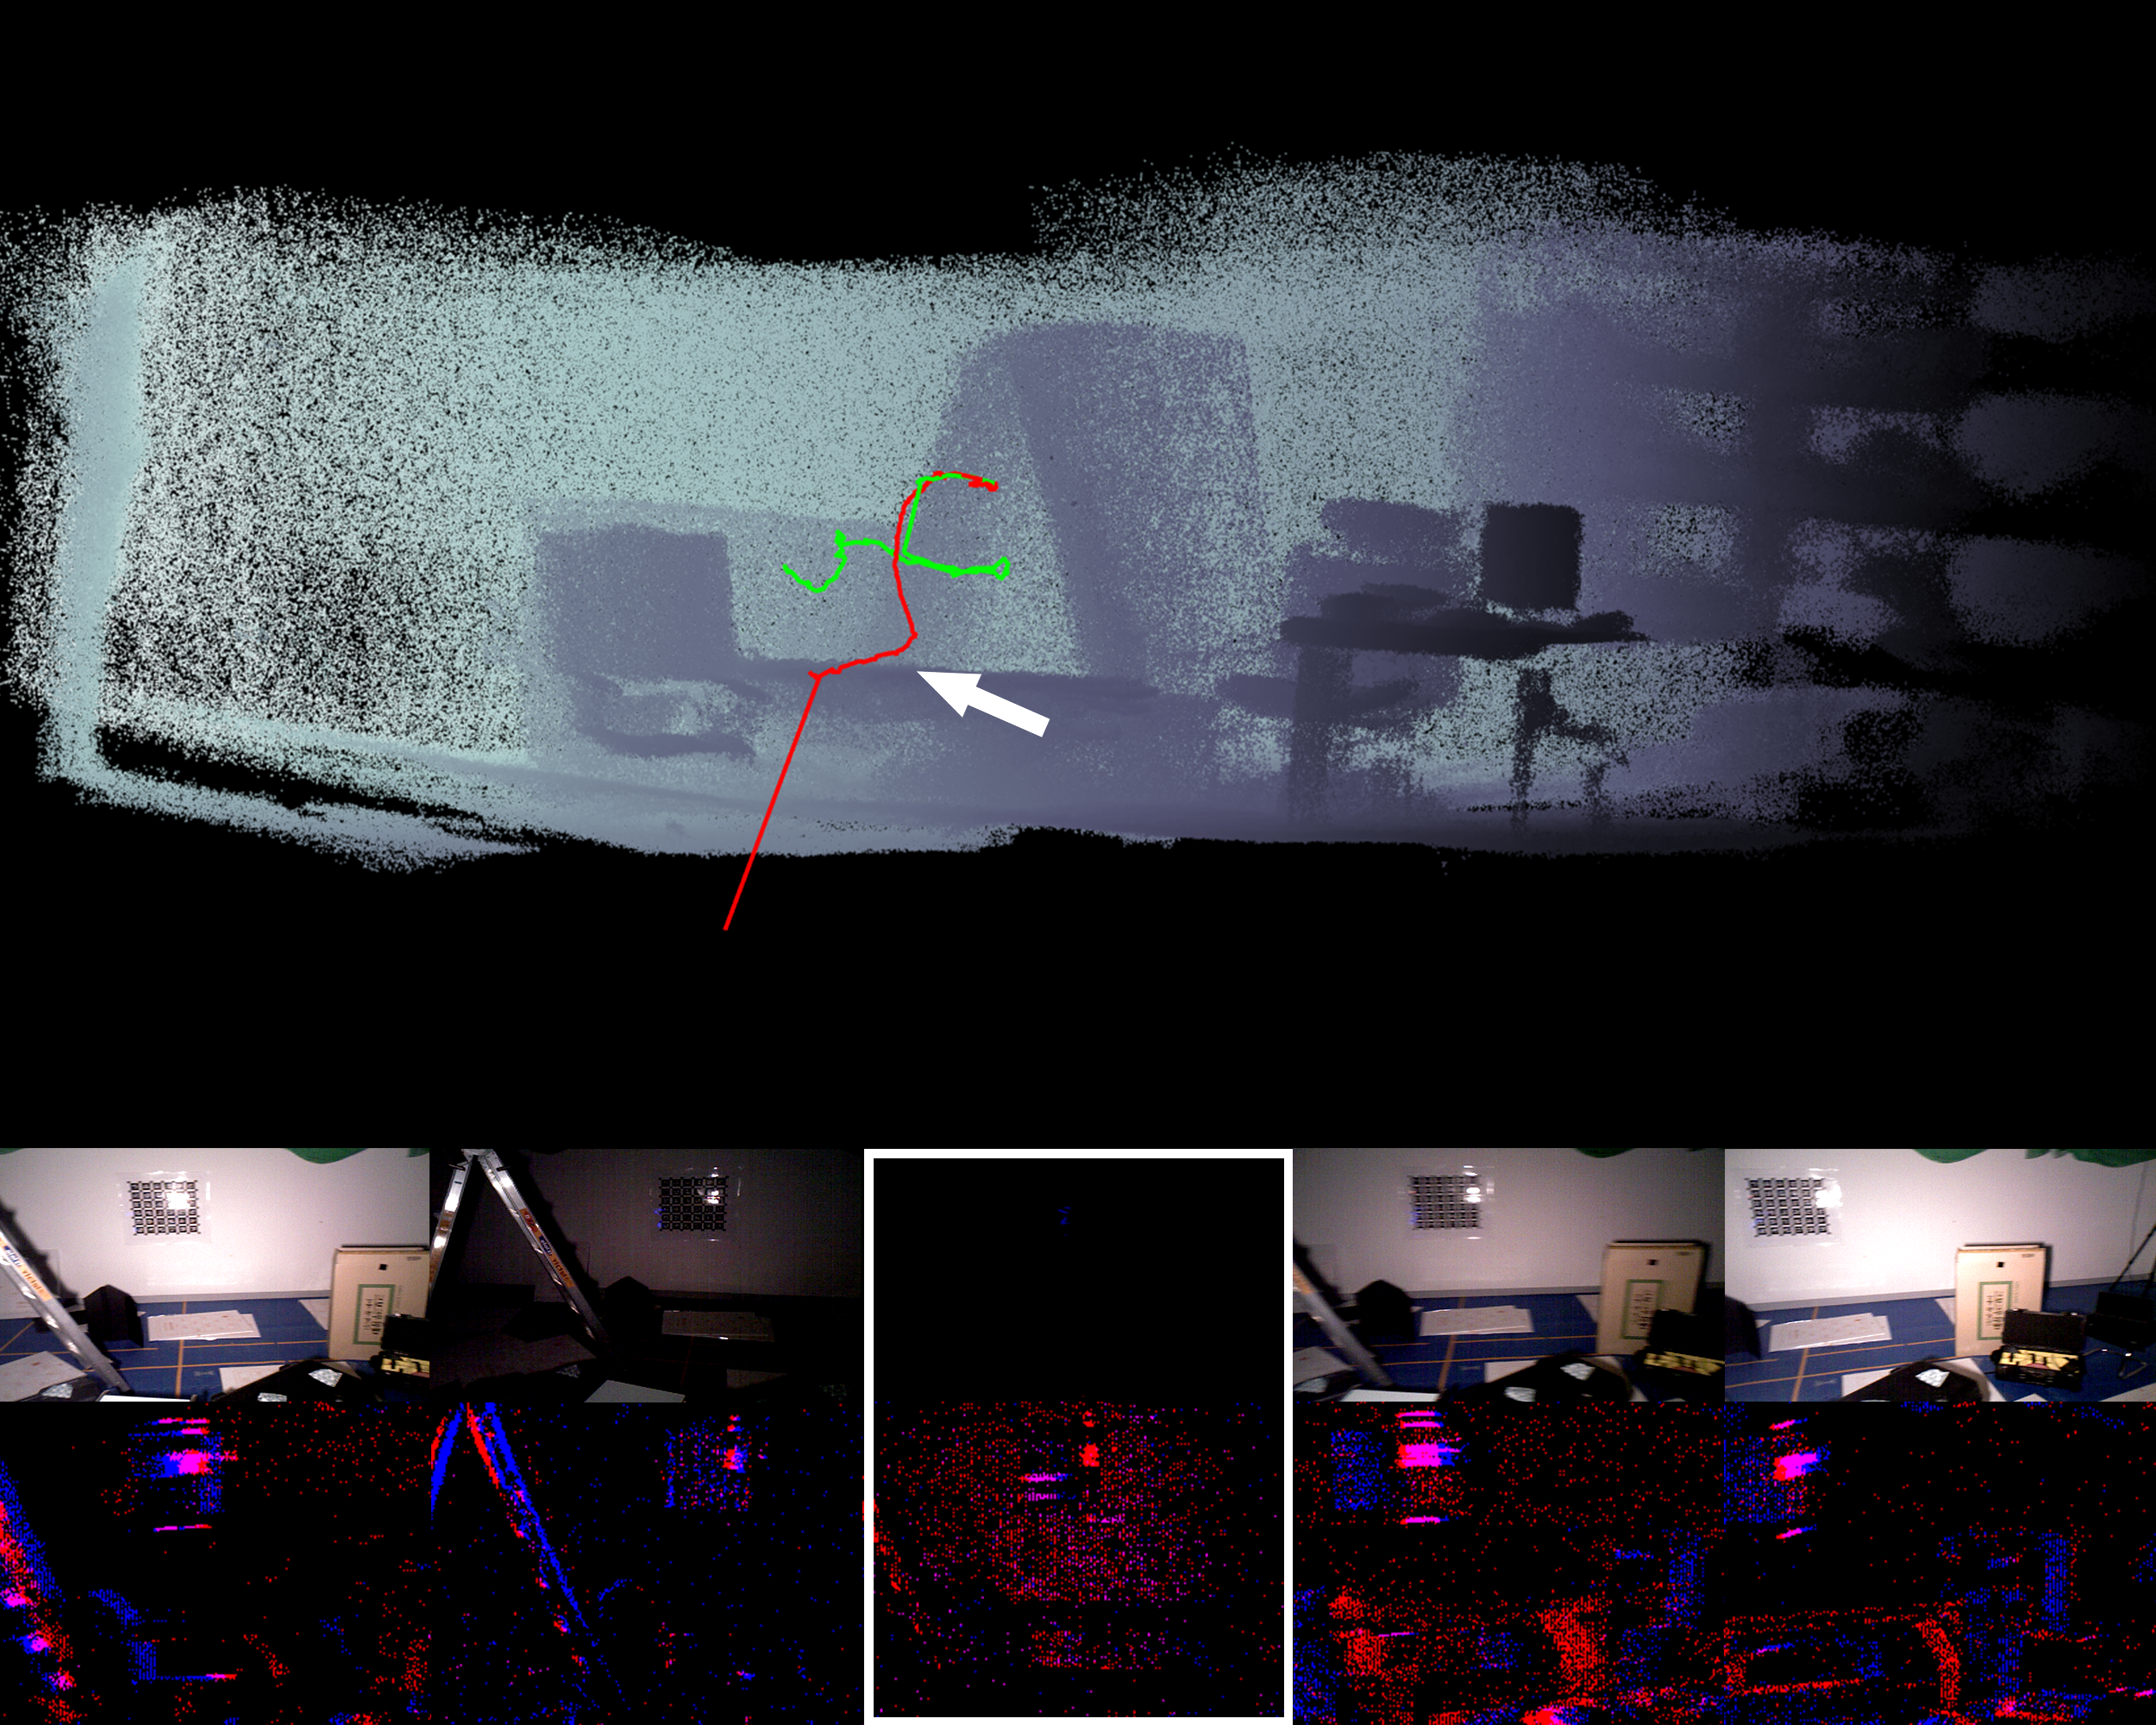
\includegraphics[width=0.86\textwidth]{figures/fig3}
	
	\caption{Estimated trajectory and reconstructed pointcloud for vivid dataset, for varying light sequence.
		As there is lighting change over time, image feature based ORB-SLAM2 (red path) fails to estimate trajectory
		when the light turns off. However, Ours (green path) succeeds on estimating the trajectory robustly under
		circumstances.}
	
	\label{fig:trajsample}
\end{figure*}


Since the resolution of DAVIS camera is relatively lower than other sensors, the output
of our algorithm does not gives better results to ORB-SLAM2, on stable environments.
In global lighting sequences the room was sufficiently bright with constant ambient
light. And for the dark and local light sequences, we ran our experiment with the
ambient light turned off. In local light sequences, only an LED installed with sensor
rig was turned on, producing unequally configured lighting profile for the scene.
As in \figref{fig:trajsample} local light source changes its brightness, and RGB-based
features fail easily, yielding tracking lost.

\section{Conclusion}

We have introduced a method to solve pose estimation problem by introducing continuous
trajectory fused with event camera, for robust convergence of slow and accurate depth sensors.
Our algorithm solves environment undersampling problem by robustly updating time-continuous
trajectory parameters to estimate poses between sparsely updated sensor measurements.
We also summarized results by showing robustness under lighting and motion variances on publicly
released dataset provided with calibration parameters and groundtruth. Our vision for visibility dataset
is the first public dataset to include three calibrated multi domain vision sensors, to provide
the standard to develop vision for visibility under real-world environments.

%\bibliographystyle{ieeetr}
\bibliographystyle{IEEEtranN} % not IEEEtran, but IEEEtranN for using citeauthor
\bibliography{string-short,iros2020-jhlee}

\end{document}
